% Figure Q2, generated by experiments/q2_convergence_trajectories.py.
\begin{figure}[t]
  \centering
  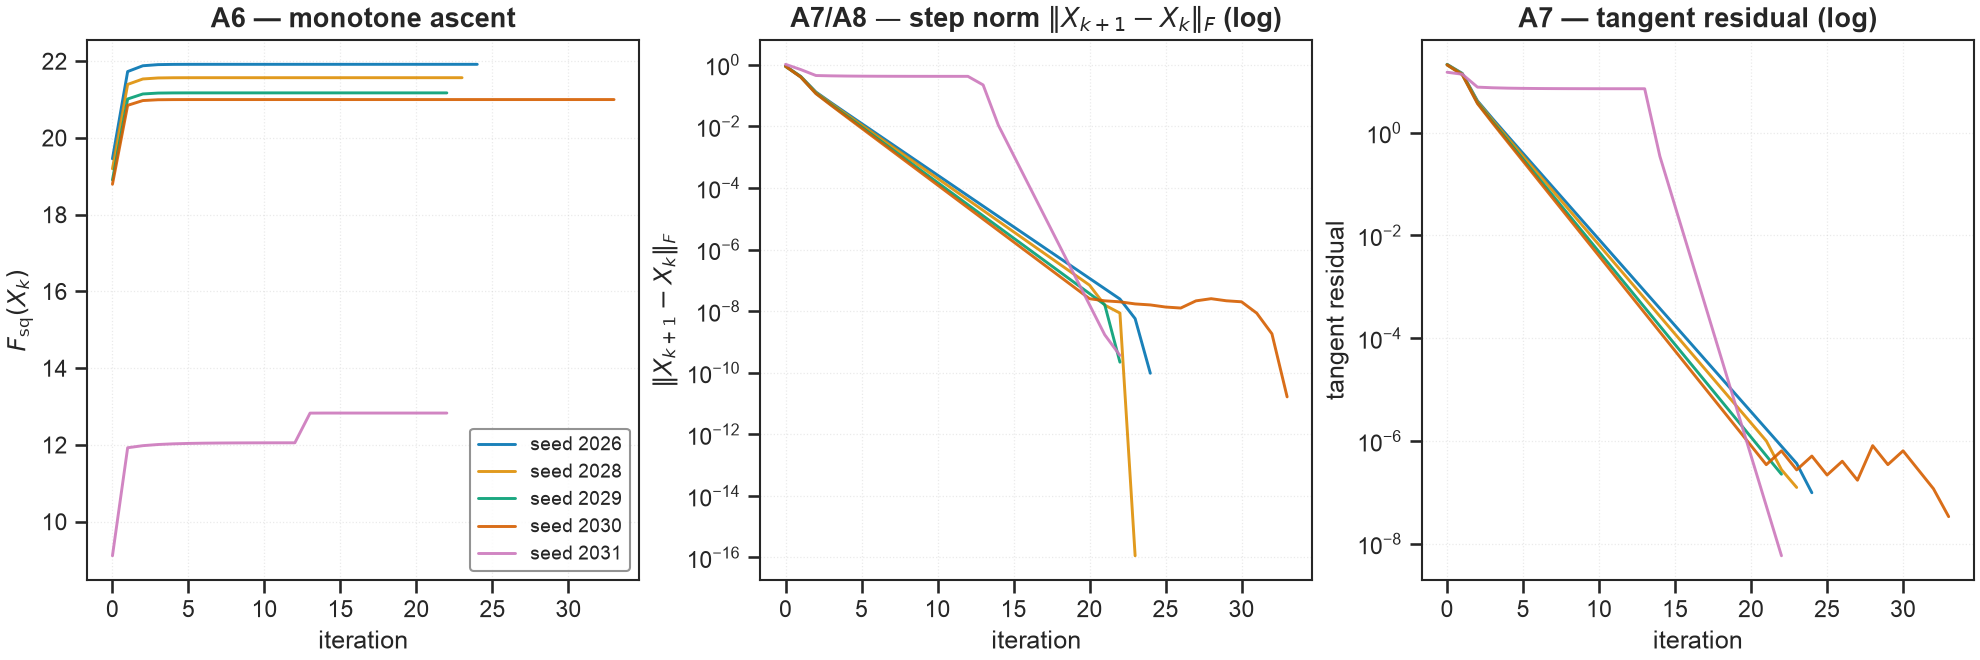
\includegraphics[width=\linewidth]{../shared/figures/generated/q2_convergence_trajectories.png}
  \caption{\textbf{Q2, safeguarded ascent trajectories on A-SQ.} Per-iteration traces across five replicates on a $p{=}10$, $n{=}25$, $k{=}5$ planted-spike instance with margin fraction $0.6$ and initial angle $0.6$~rad; one trace per colour. \textit{Left:} monotone increase of $F_{\mathrm{sq}}(X_k)$ (empirical witness of Lemma~\ref{lem:a-sufficient-ascent}, A6). \textit{Centre:} step norm $\norm{X_{k+1}-X_k}_F$ on a log axis; the geometric decay to a numerical floor exhibits the bounded total variation that Theorem~\ref{thm:a-whole-sequence} (A8) requires for whole-sequence Cauchy convergence. \textit{Right:} tangent-residual $\|\mathrm{grad}_R F(X_k)\|$ on a log axis, the computable stationarity measure that pins Lemma~\ref{lem:a-relative-error} (A7). Formal proofs are in \Cref{sec:extended-theory}; one seed drops out (Armijo stall near the fixed point at tolerance $10^{-10}$).}
  \label{fig:q2-trajectories}
\end{figure}
